\section{Durchführung der Spektrumanalyse}
Zunächst wird die Spektrumanalyse mithilfe von Fieldfox Spectrum Analyzer durchgeführt. Für eine sinnvolle Analyse wird die ResBW auf 1 kHz eingestellt, um eine ausreichende Auflösung zu gewährleisten.
Obwohl die Startfrequenz für die Analyse auf 1,248 GHz und die Stopfrequenz auf 1,252 GHz gesetzt werden sollte, liegt die tatsächliche Trägerfrequenz der Platine selbst bei 1,200 GHz. Deswegen wird die Startfrequenz auf 1,198 GHz und die Stopfrequenz auf 1,202 GHz gesetzt. 
\section{Sender mit und ohne Datenübertragung}
Die Messung des Spektrums erfolgt in zwei Szenarien: Zunächst wird der Sender ohne Datenübertragung betrieben, um das Grundrauschen und die Trägerfrequenz zu erfassen. Anschließend wird der Sender mit aktivierter Datenübertragung betrieben, um die Auswirkungen der Modulation auf das Spektrum zu beobachten.

Die Sendeplatine wird zuerst an die Versorgungsspannung angeschlossen, um den Sender zu aktivieren. Es wird eine SMA-Verbindung mit dem Fieldfox hergestellt, um das Rauschen zu minimieren. Ein nichtqualitatives Bild der Versuchanseinrichtung ist in Abbildung~\ref{fig:Versuchsanordnung} zu sehen.

    \subsection{Messung ohne Datenübertragung}
    Erstens soll die Messung ohne Datenübertragung durchgeführt werden. Hierdurch wird die Trägerfrequenz und das Grundrauschen des Senders erfasst. Diese Messung dient als Referenz für die spätere Analyse der Modulationseffekte.
    \begin{figure}[H]
        \centering
        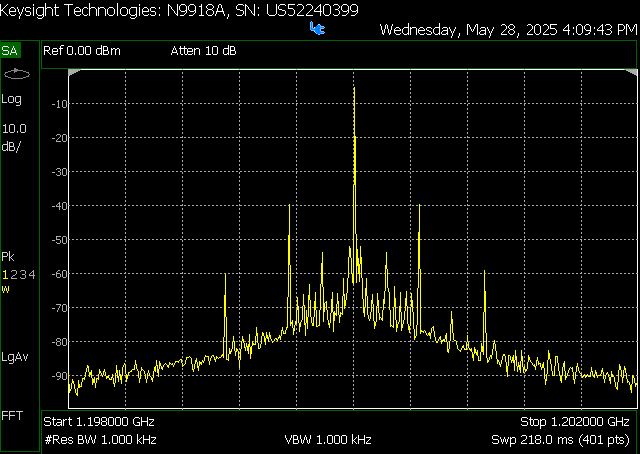
\includegraphics[width=0.8\textwidth]{Pictures/4.4.png}
        \caption{Frequenzspektrum des Senders ohne Datenübertragung}
        \label{fig:OhneDaten}
    \end{figure}
    \subsection{Messung mit Datenübertragung}
    Zweitens soll die Messung mit Datenübertragung durchgeführt werden. Die Effekte der Modulation auf das Frequenzspektrum werden hierdurch sichtbar. Die Modulation verändert die Amplitude und Frequenz des Signals, was zu einer breiteren Verteilung im Frequenzspektrum führt.
    Die Anwendung HTerm bietet die Möglichkeit, die Daten mit einer variablen Baudrate zu übertragen. In diesem Versuch wurde die Messung bei einigen der zur Auswahl stehenden Baudraten durchgeführt, um die Auswirkungen der Datenrate auf das Frequenzspektrum zu untersuchen. Diese Baudraten sind 1200 Baud, 57600 Baud, 115200 Baud, 128000 Baud und 256000 Baud.
    Hierbei ist zu beachten, dass die Baudrate von 115200 eine gängige Rate für Mikrocontroller-Kommunikation ist und in vielen Anwendungen verwendet wird.


    \begin{figure}[H]
        \centering
        \begin{minipage}{0.47\textwidth}
            \centering
            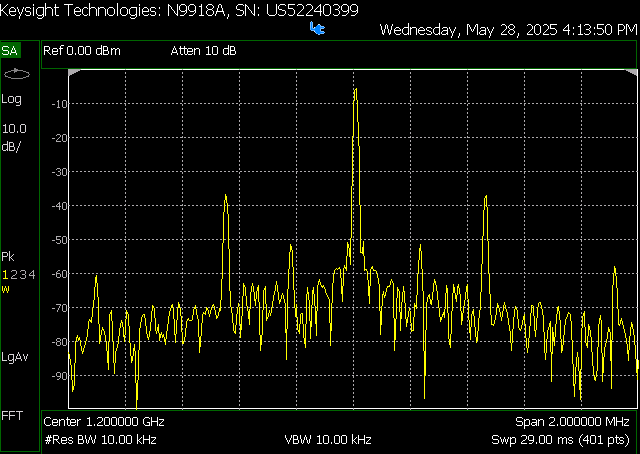
\includegraphics[width=0.8\textwidth]{Pictures/4.4C.1200.png}
            \caption*{1200 Baud}
        \end{minipage}
        \hfill
        \begin{minipage}{0.47\textwidth}
            \centering
            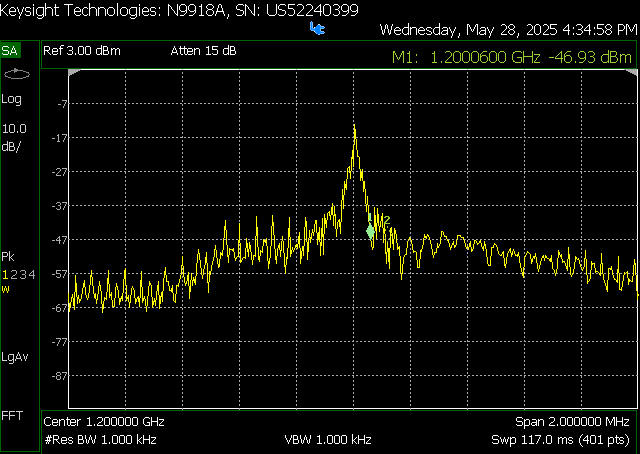
\includegraphics[width=0.8\textwidth]{Pictures/4.4C.57600.png}
            \caption*{57600 Baud}
        \end{minipage}

        \vspace{0.5cm}

        \begin{minipage}{0.47\textwidth}
            \centering
            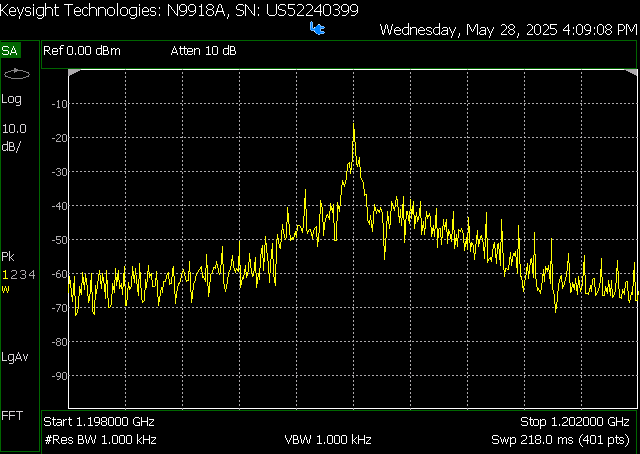
\includegraphics[width=0.8\textwidth]{Pictures/4.4C.115200.png}
            \caption*{115200 Baud}
        \end{minipage}
        \hfill
        \begin{minipage}{0.47\textwidth}
            \centering
            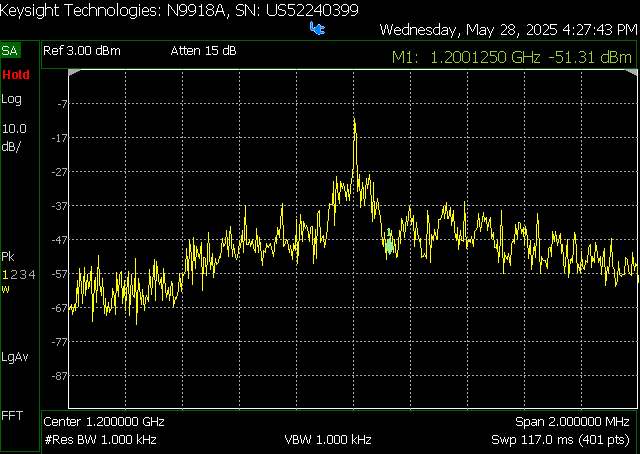
\includegraphics[width=0.8\textwidth]{Pictures/4.4C.128000.png}
            \caption*{128000 Baud}
        \end{minipage}

        \vspace{0.5cm}
        \begin{minipage}{0.1\textwidth}
            % Empty minipage for centering
        \end{minipage}
        \hfill
        \begin{minipage}{0.47\textwidth}
            \centering
            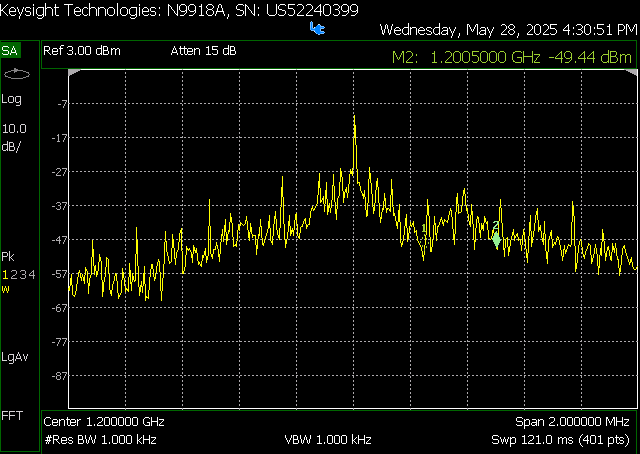
\includegraphics[width=0.8\textwidth]{Pictures/4.4C.256000.png}
            \caption*{256000 Baud}
        \end{minipage}
        \hfill
        \begin{minipage}{0.1\textwidth}
            % Empty minipage for centering
        \end{minipage}

        \caption{Frequenzspektrum des Senders mit Datenübertragung bei verschiedenen Baudraten.}
        \label{fig:MitDaten}
    \end{figure}

Anhand der Ergebnisse in Abbildung~\ref{fig:MitDaten} im Vergleich zur Abbildung~ref{fig:OhneDaten} auf, dass es sich bei unserem Versuch um Amplitudenmodulation handelt, da die Amplitude der Trägerfrequenz bei der Datenübertragung nicht konstant bleibt. Diese variiert in Abhängigkeit von der übertragenen Information. Die Frequenz bleibt jedoch konstant, was ein typisches Merkmal der Amplitudenmodulation ist.
\section{Vergleich mit den theoretischen Reflexionen}



\section{Variation der Datenrate}
\section{Aufbau und Funktionsweise des Demodulators}
blabla
\clearpage